\documentclass[a4paper]{article}

\usepackage{graphicx}
\usepackage{lastpage}
\usepackage{fancyhdr}
\pagestyle{fancy}

\addtolength{\oddsidemargin}{-.875in}
\addtolength{\evensidemargin}{-.875in}
\addtolength{\headwidth}{1.75in}
\addtolength{\textwidth}{1.75in}

\lhead{Gareth Pulham}
\rhead{40099603}
\lfoot{MEng Software Engineering}
\cfoot{\today}
\rfoot{\thepage\ of \pageref{LastPage}}

\begin{document}
    \begin{titlepage}
        \title{SOC10101 Week 9 Report}
        \author{Gareth Pulham, 40099603}
        \date{\today}
        \maketitle
        \thispagestyle{empty}
    \end{titlepage}

    \tableofcontents

    \section{Project Aims and Objectives}
    \begin{itemize}
        \item To investigate different methods to accelerate radio viewshed calculations (RVC)
        \item To implement and compare selected methods between CPU and GPU accelerated versions
    \end{itemize}

    \section{Introduction}
    Radio viewsheds are the area of terrain that a given emitter's signals can be received from. The calculation of
    these viewsheds are as a result critical to the planning of radio networks and the placement of individual masts
    and emitters. While the general public are mostly unaware of radio networks that exist in the UK beyond broadcast
    FM and cellular telephony, they have reach into many fields such as TV, rural community broadband, WANs for
    individual organisations, etc. Because of this, tools have been developed in many geographical information systems
    to calculate them, however they tend to be slow, calculated in series on the CPU. The intention of this project is
    to investigate, implement, and compare GPU acceleration of RVCs to present implementations and tools.

    \section{Schedule and Plan}
    \begin{itemize}
        \item October, end - Infrastructure and tools complete (Complete)
        \item November, end - Week 9 Report/Second marker review (In progress)
        \item November, end - CPU implementation of RVC (In progress)
        \item December, end - GPU implementation of RVC
        \item January, beginning - Begin dissertation
        \item February - Final changes to implementation and benchmarking
        \item March - Dissertation complete
        \item March - Poster design
        \item April - Viva
        \item April - Poster presentation
    \end{itemize}

    \section{Approaches and Techniques}
    To begin, time was invested investigating different ways to calculate RVCs. The three prominent techniques
    investigated were heat-diffusion pathfinding, raytracing, and line sweeping.

    Diffuse pathfinding was soon discarded from consideration: built mainly for GPU accelerating pathfinding, it would
    allow beams to curve unrealistically around objects. One implementation however does demonstrate the use of dynamic
    parallelism, which may be a useful path to research in aiding the calculation of fresnel zones later in my work.

    Ray tracing is the most likely form of implementation for this project - it is simple, well understood, and well
    suited to the task. Additionally, applied to the problem and data at hand it is embarrassingly parallel, meaning
    that the potential speedup is great compared to CPU based calculations.

    An additional technique would be line sweeping. Line sweeping is an algorithm where only interesting points are
    calculated, and the rest discarded as obviously unreachable (i.e., in the shadow of another point). This is the
    approach taken by Grass GIS's \texttt{r.viewshed} function (https://grass.osgeo.org/grass73/manuals/r.viewshed.html)
    , and a similar technique is documented at Red Blob Games (http://www.redblobgames.com/articles/visibility/). This
    technique can be significantly faster on the CPU as it can ignore a number of cells at a cheaper cost than
    calculating them individually. This may not hold true on the GPU as it introduces data dependency where a cell may
    or may not be skipped based on the results of another cell.

    \section{Prior Art}
    To find what solutions, if any, existed already in this space, previous RVC implementations were investigated.
    The findings are listed below.

        \subsection{HeyWhatsThat}
        HeyWhatsThat (http://www.heywhatsthat.com/) is a web-based horizon and viewshed tool designed for hikers who
        want to identify what can be seen from (typically) a mountain peak. Additonal services are offered such as
        route profiling and multi-point viewshed calculations.

        Notably, HWT includes options specific to RVCs rather than just visible like horizon/viewshed, with options to
        calculate fresnel zones on specific cross sections of the viewshed.

        HWT has a technical FAQ where they discuss some of the implementation details and the data sources they have
        used (specifically, the SRTM dataset, which has a resolution of 30m in US/Australia and 90m elsewhere), but is
        also a good introduction to viewshed calculation in general.

        Key points:
        \begin{itemize}
            \item Closed source, difficult to build into other tools
            \item Non-accelerated
        \end{itemize}

        \subsection{POV-Ray}
        POV-Ray (http://www.povray.org/) is the Persistence Of Vision Raytracer. Primary this tool is designed for
        rendering scenes build by 3D modellers, but it has been used previously by the Tegola project to calculate
        RVCs by combining height data with OS maps, and then using light sources to act as emitters, though the project
        admits a number of drawbacks with their method (http://www.tegola.org.uk/2013/03/24/pretty-pictures.html).

        Additionally, POV-Ray is not GPU accelerated (http://www.povray.org/documentation/view/3.6.0/182/).

        Key points:
        \begin{itemize}
            \item Requires significant manual work on account of primarily being a scene renderer
            \item Non-accelerated
        \end{itemize}

        \subsection{ArcGIS}
        esri's ArcGIS plaform is a leading product in the GIS market. Initially released in 1999, it was estimated in
        2010 that esri controls 40\% of the GIS market
        (http://www.esri.com/news/releases/11-4qtr/arc-advisory-group-report-esri-a-leading-gis-provider-in-utilities-sector.html).

        ArcGIS is a commerical product with a number of features not available in the base versions, and 3D surface
        tools such as Viewshed and Viewshed 2 require additional licensing
        (http://desktop.arcgis.com/en/arcmap/10.3/tools/spatial-analyst-toolbox/viewshed-2.htm).

        However, ArcGIS is one of the few products in the market that does support GPU acceleration, not just as a
        principle but in practice, including the Viewshed 2 function. On the flip side, this acceleration is
        specifically nvidia, AMD and Intel cards are not supported.

        Key points:
        \begin{itemize}
            \item Commercial
            \item Windows only
        \end{itemize}

        \subsection{GRASS GIS}
        GRASS GIS, initially developed by the US Army, has developed into a highly extensible, open source GIS system.
        With over 350 core modules and more than 100 user developed extensions covering almost every GIS function,
        including viewshed calculations (https://grass.osgeo.org/grass73/manuals/r.viewshed.html).

        GRASS has also been building in GPU acceleration (https://grasswiki.osgeo.org/wiki/GPU), though at present
        little appears to have been implemented and integrated into the main release.

        Key points:
        \begin{itemize}
            \item Non-accelerated (has acceleration for r.viewshed on its ``of-interest'' list)
        \end{itemize}

        \subsection{QGIS}
        QGIS (previously Quantim GIS) is a cross-platform GIS tool based on the Qt framework.

        QGIS doesn't at present have a bundled viewshed tool, however, plugins are available
        (https://plugins.qgis.org/plugins/ViewshedAnalysis/).

        Additionally, at this point, QGIS has no GPU acceleration, although individual plugins are free to call out to
        GPUs on their own.

        Key points:
        \begin{itemize}
            \item Plugin available
            \item Non-accelerated
        \end{itemize}

    \section{Current situation}
    Presently, the project is about half way through the implementation phase. Tooling and common code has mostly been
    written, such as visualisers and parsers for the file format used by EDINA (https://en.wikipedia.org/wiki/EDINA) to
    distribute heightmap rasters produced by the Ordnance Survey.

    Specifically at this point:
    \begin{itemize}
        \item Common data structures such as heightmap and viewshed types
        \item Common data structure manipulations such as reading and writing the above types to file, and the
            automatic creation of the appropriate shape of structure from the attributes of another
        \item CPU only implementations of map manipulations such as deforming heightmaps to the earths curvature, as
            well as a CPU only implementation for viewshed analysis
        \item Tests for all the above
        \item Visualisation tools to view heightmaps coloured by visibility
    \end{itemize}

    \begin{figure}[!h]
        \centering
        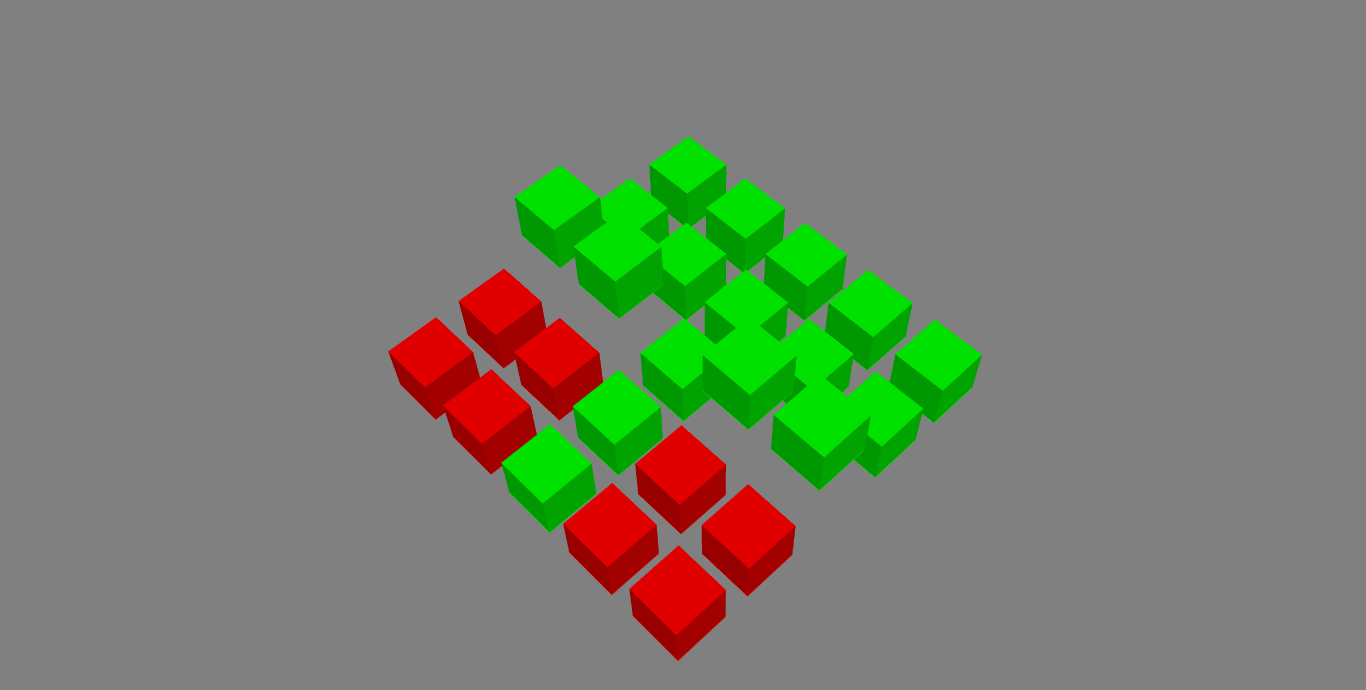
\includegraphics[width=\textwidth]{images/demo_render.png}
        \caption{Example rendering of a small (5x5) heightmap}
    \end{figure}
\end{document}
